\documentclass[letterpaper]{article}


\usepackage{amsmath,amsfonts,amsthm} % Math packages
\usepackage[margin = 1in]{geometry}
\usepackage{tikz} %for the GUI
\usepackage{graphicx}

\begin{document}

\section{Ideas}

\subsection{Initial}


\begin{itemize}
   \item Purchase Raspberry Pi Zero
   \item Purchase Nordic Semiconductor ANT+ chip
   \item General steps
   \begin{enumerate}
      \item Purchase ANT+ Chip
      \item Work to adapt a C++ ANT+ library to receive data stream from peripheral devices
      \item Implement calculations and cycling features
      \item Design the user interface using QT Creator
      \item Assemble the hardware  
   \end{enumerate}
\end{itemize}


\section{Features}
\begin{itemize}
   \item CP curve
   \begin{itemize}
      \item Curve fit
      \item Data file with best power for ever interval
   \end{itemize}
   \item W' implementation
\end{itemize}



\section{Screen Choice}
On screen choice, I think it will decide how we interact with the device. Basically, whether or not it is a touch screen. An additional note: displays can interact with an RPi with either the GPIO pins or a serial display output. I think we need to use the serial display output to free up the GPIO for any other devices. The touch screen I have uses GPIO which would make this hard. 

\begin{itemize}
   \item Touch screen
      \begin{itemize}
         \item Resistive
         \item Capacitive - \textbf{NO}
      \end{itemize}
   \item Just normal screen with buttons
\end{itemize}

\section{Graphical User Interface}

\begin{figure}[!htb]
\centering
\begin{minipage}{.49\textwidth}
\centering
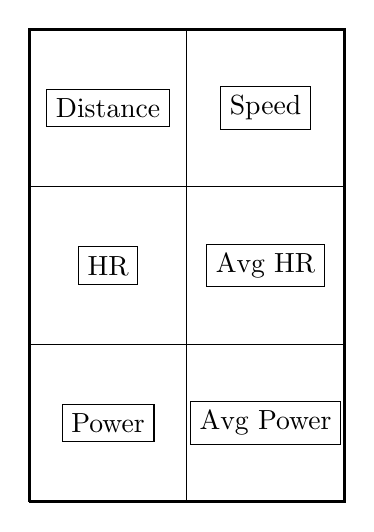
\begin{tikzpicture}
\draw[very thick] (0,0) -- (4,0) -- (4,6) -- (0,6) -- (0,0);
\draw (0,2) -- (4,2);
\draw (0,4) -- (4,4);
\draw (2,0) -- (2,6);
\node[draw] at (1,1) {Power};
\node[draw] at (3,1) {Avg Power};
\node[draw] at (1,3) {HR};
\node[draw] at (3,3) {Avg HR};
\node[draw] at (1,5) {Distance};
\node[draw] at (3,5) {Speed};
\end{tikzpicture}

\caption{Home page}
\end{minipage} \hfill
\begin{minipage}{.49\textwidth}
\centering
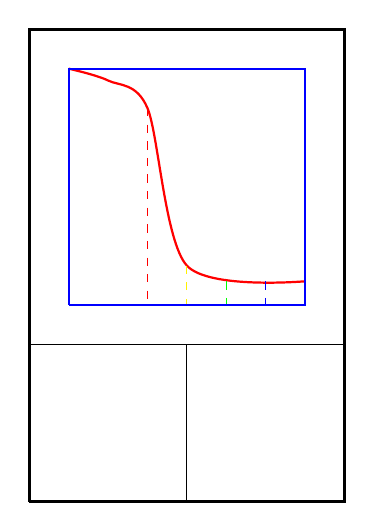
\begin{tikzpicture}
\draw[very thick] (0,0) -- (4,0) -- (4,6) -- (0,6) -- (0,0);
\draw (0,2) -- (4,2);
\draw (2,0) -- (2,2);
\draw [red,thick] plot [smooth] coordinates {(.5,5.5) (1,5.35) (1.5,5) (2,3) (3.5,2.8)};
\draw[dashed,red] (1.5,5) -- (1.5, 2.5);
\draw[dashed,yellow] (2,3) -- (2, 2.5);
\draw[dashed,green] (2.5,2.8) -- (2.5, 2.5);
\draw[dashed,blue] (3,2.8) -- (3, 2.5);
\draw[blue, thick] (.5,2.5) -- (3.5,2.5) -- (3.5,5.5) -- (.5,5.5) -- (.5,2.5);
\end{tikzpicture}

\caption{CP}
\end{minipage}
\end{figure}

\end{document}
